%=================================================================
% SAD - Documento de Arquitectura de Software
% Proyecto Tickets-NFT B2B (Stellar/Soroban)
%=================================================================
\documentclass[12pt,oneside]{article}

% ====== Paquetes y formato ======
\usepackage[spanish,es-nodecimaldot]{babel}
\usepackage[utf8]{inputenc}
\usepackage[T1]{fontenc}
\usepackage[a4paper,margin=2.5cm]{geometry}
\usepackage{setspace}
\onehalfspacing
\usepackage{graphicx}
\usepackage{float}
\usepackage{hyperref}
\hypersetup{
  colorlinks=true,
  linkcolor=blue,
  urlcolor=blue,
  citecolor=black,
  pdfauthor={Grupo 12},
  pdftitle={SAD - Proyecto Tickets-NFT B2B}
}
\usepackage{booktabs}
\usepackage{tabularx}
\usepackage{longtable}
\usepackage{array}
\usepackage{enumitem}
\setlist[itemize]{left=0pt,label=--,itemsep=2pt,topsep=4pt}
\setlist[enumerate]{left=0pt,itemsep=2pt,topsep=4pt}
\setcounter{secnumdepth}{3}
\setcounter{tocdepth}{3}
\usepackage{listings}
\usepackage{xcolor}
\usepackage{amssymb}

% Configuración de listings para código
\lstset{
  basicstyle=\ttfamily\small,
  breaklines=true,
  frame=single,
  numbers=left,
  numberstyle=\tiny\color{gray},
  keywordstyle=\color{blue},
  commentstyle=\color{green!60!black},
  stringstyle=\color{red!70!black},
  tabsize=2
}

% ====== Metadatos del proyecto ======
\newcommand{\projectname}{Reventa B2B de tickets con NFTs en Stellar (Soroban)}
\newcommand{\shortname}{Proyecto Tickets-NFT B2B}
\newcommand{\version}{0.1}
\newcommand{\docdate}{\today}
\newcommand{\course}{Trabajo de Grado -- Ingeniería de Sistemas}
\newcommand{\team}{Grupo 12}

% ====== Documento ======
\begin{document}

% ====== Portada ======
\begin{titlepage}
  \centering
  {\Large Documento de Arquitectura de Software (SAD)\par}
  \vspace{1.2cm}
  {\huge \textbf{\projectname}\par}
  \vspace{0.3cm}
  {\Large (\shortname)\par}
  \vspace{1.2cm}
  {\large Versión 0.3 — \docdate\par}
  \vspace{0.8cm}
  
\includegraphics[width=4cm]{pontificia-universidad-javeriana-seeklogo.png}\par
  \vspace{0.4cm}
  {\Large Pontificia Universidad Javeriana Bogotá\par}
  \vfill
  {\large \course\par}
  \vspace{0.3cm}
  {\large Director: Rafael Vicente Paéz Méndez, PhD\par}
  \vspace{0.3cm}
  {\large Cliente: B.A.F: Blockchain Acceleration Foundation\par}
  \vfill
  {\large\textbf{Autores:}\par}
  {\large
    Juan Diego Arias Durán\\
    Santiago Andrés Mesa Niño\\
    Andrés Felipe Manosalva Garzón\\
    Juan Camilo Carvajal Rodríguez\par}
  \vspace{1cm}
\end{titlepage}

% ====== Preliminares ======
\pagenumbering{roman}

% ------ Historial de cambios ------
\section*{Historial de cambios}
\begin{longtable}{@{}p{2cm} p{3cm} p{7.5cm} p{2.5cm}@{}}
  \toprule
  \textbf{Versión} & \textbf{Fecha} & \textbf{Descripción} & \textbf{Autor(es)}\\
  \midrule
  \endfirsthead
  \toprule
  \textbf{Versión} & \textbf{Fecha} & \textbf{Descripción} & \textbf{Autor(es)}\\
  \midrule
  \endhead
  \bottomrule
  \endfoot
  0.1 & 10/03/2026 & Versión inicial del SAD: estructura base del documento. & \team\\
  0.2 & 13/03/2026 & Desarrollo de las secciones 1 (Introducción), 2 (Representación arquitectónica) y 3 (Objetivos y restricciones arquitectónicas). & \team\\
  0.3 & 15/03/2026 & Desarrollo de las secciones 4 (Vista de casos de uso), 5 (Vista lógica) y 6 (Vista de procesos). & \team\\
\end{longtable}

\newpage

% ------ Índices ------
\tableofcontents
\newpage
\listoffigures
\listoftables
\clearpage

% ====== Cuerpo ======
\pagenumbering{arabic}

%===============================================================
\section{Introducción}
\label{sec:introduccion}
%===============================================================

\subsection{Propósito}
\label{subsec:proposito}

Este documento describe la \textbf{arquitectura de software} del sistema \textbf{\shortname}. Su propósito es:

\begin{itemize}
  \item Comunicar las decisiones arquitectónicas fundamentales del sistema a todos los interesados.
  \item Servir como referencia técnica para el equipo de desarrollo durante la implementación.
  \item Documentar las vistas arquitectónicas que permiten comprender la estructura, comportamiento y despliegue del sistema.
  \item Justificar las decisiones de diseño y los \textit{trade-offs} realizados.
\end{itemize}

\subsection{Alcance}
\label{subsec:alcance}

El SAD abarca la arquitectura del prototipo académico del sistema de reventa B2B de tickets con NFTs sobre Stellar (Soroban), incluyendo:

\begin{itemize}
  \item El contrato inteligente Soroban (lógica on-chain).
  \item El backend/API que interactúa con el contrato.
  \item El frontend web de demostración.
  \item Las integraciones con la red Stellar (testnet).
\end{itemize}

\subsection{Definiciones, acrónimos y abreviaturas}
\label{subsec:definiciones}

\begin{longtable}{@{}p{3.5cm} p{11cm}@{}}
  \toprule
  \textbf{Término} & \textbf{Definición}\\
  \midrule
  \endhead
  \bottomrule
  \endfoot
  SAD & \textit{Software Architecture Document}. Este documento.\\
  NFT & \textit{Non-Fungible Token}. Activo digital único que representa un ticket en blockchain.\\
  Stellar & Red blockchain orientada a pagos y emisión de activos digitales.\\
  Soroban & Plataforma de contratos inteligentes sobre Stellar, basada en WebAssembly (Wasm).\\
  WASM & \textit{WebAssembly}. Formato de bytecode al que se compilan los contratos Soroban.\\
  B2B & \textit{Business to Business}. Modelo de negocio del sistema.\\
  API & \textit{Application Programming Interface}.\\
  REST & \textit{Representational State Transfer}. Estilo arquitectónico para APIs web.\\
  Testnet & Red de pruebas de Stellar sin valor monetario real.\\
  SRS & \textit{Software Requirements Specification}. Documento de requerimientos del proyecto.\\
  SPMP & \textit{Software Project Management Plan}. Plan de gestión del proyecto.\\
\end{longtable}

\subsection{Referencias}
\label{subsec:referencias}

\begin{enumerate}[leftmargin=*,label={[\arabic*]}]
  \item IEEE Std 1471-2000: \textit{IEEE Recommended Practice for Architectural Description of Software-Intensive Systems}.
  \item ISO/IEC/IEEE 42010:2011: \textit{Systems and software engineering — Architecture description}.
  \item Brown, S. (2018). \textit{The C4 Model for Visualising Software Architecture}. \url{https://c4model.com/}.
  \item Bass, L., Clements, P., \& Kazman, R. (2012). \textit{Software Architecture in Practice}, 3rd Edition. Addison-Wesley.
  \item SRS del sistema Tickets-NFT B2B (v0.1).
  \item SPMP del sistema Tickets-NFT B2B (v1.1).
  \item Stellar Development Foundation: \textit{Stellar Documentation}, \url{https://developers.stellar.org/}.
  \item Soroban Documentation: \textit{Smart Contracts on Stellar}, \url{https://soroban.stellar.org/}.
\end{enumerate}

\newpage
\subsection{Visión general del documento}
\label{subsec:vision-general}

El resto del documento se organiza así:

\begin{itemize}
  \item \textbf{Sección~\ref{sec:representacion}}: describe el modelo arquitectónico utilizado y las vistas que se presentan.
  \item \textbf{Sección~\ref{sec:objetivos-restricciones}}: enumera los objetivos y restricciones arquitectónicas.
  \item \textbf{Sección~\ref{sec:vista-casos-uso}}: vista de casos de uso.
  \item \textbf{Sección~\ref{sec:vista-logica}}: vista lógica (paquetes, clases, capas).
  \item \textbf{Sección~\ref{sec:vista-procesos}}: vista de procesos (concurrencia, flujos).
  \item \textbf{Sección~\ref{sec:vista-despliegue}}: vista de despliegue (infraestructura física/virtual).
  \item \textbf{Sección~\ref{sec:vista-implementacion}}: vista de implementación (componentes, módulos).
  \item \textbf{Sección~\ref{sec:vista-datos}}: vista de datos (modelo de datos on-chain y off-chain).
  \item \textbf{Sección~\ref{sec:calidad}}: atributos de calidad y tácticas arquitectónicas.
  \item \textbf{Sección~\ref{sec:decisiones}}: registro de decisiones arquitectónicas (ADRs).
\end{itemize}

%===============================================================
\newpage
\section{Representación arquitectónica}
\label{sec:representacion}
%===============================================================

La arquitectura de Stellar Tickets se describe mediante el modelo \textbf{C4} de Simon Brown, que provee niveles de abstracción progresivos (contexto, contenedores, componentes, código) para comunicar la arquitectura a audiencias con distintos niveles de detalle técnico. Este modelo es especialmente adecuado para sistemas híbridos como el presente, donde la lógica se distribuye entre contratos inteligentes on-chain y servicios convencionales off-chain.

\subsection{Niveles C4 utilizados}

Se utilizan los dos primeros niveles del modelo C4:

\subsubsection{Nivel 1 -- Contexto del sistema}

En el modelo C4, el diagrama de contexto es el nivel de abstracción más alto. Su objetivo es responder a la pregunta: \textit{¿qué es el sistema y quién interactúa con él?} No muestra detalles técnicos internos, sino que ubica al sistema como una caja negra dentro de su entorno, identificando las personas que lo usan y los sistemas externos de los que depende o con los que se comunica.

La Figura~\ref{fig:c4-contexto} presenta el diagrama de contexto de Stellar Tickets.

\begin{figure}[H]
  \centering
  
\includegraphics[width=0.7\textwidth]{contextoSecureTicket.png}
  \caption{Diagrama C4 Nivel 1 -- Contexto del sistema Stellar Tickets}
  \label{fig:c4-contexto}
\end{figure}

\paragraph{Interpretación del diagrama.} El sistema central es el \textbf{Smart Contract} desplegado en Soroban, que gestiona la validación y reventa de tickets. Alrededor de él se identifican cinco actores:

\begin{itemize}
  \item \textbf{Organizador} (empresa de boletería como TuBoleta o TicketMaster): inicializa el contrato para un evento específico, crea los tickets y los lista para venta. Sus transacciones se envían firmadas a través de la red Stellar.
  \item \textbf{Comprador} (usuario final): compra, revende y canjea tickets interactuando con el contrato a través del marketplace web. Utiliza una wallet digital no-custodial para firmar cada transacción, garantizando que solo él puede autorizar movimientos de sus activos.
  \item \textbf{Personal del evento}: consulta y verifica el estado de un ticket en el punto de acceso al evento (puerta), determinando si es válido y no ha sido consumido previamente.
  \item \textbf{Administradores SecureTicket} (equipo técnico de la plataforma): despliegan los contratos en la red Stellar, configuran las comisiones de la plataforma y mantienen la infraestructura operativa.
  \item \textbf{Wallet Digital} (Freighter): sistema externo que gestiona las claves privadas de organizadores y compradores. Toda firma de transacciones se realiza en este componente externo, lo que significa que la plataforma nunca tiene acceso a las claves de los usuarios (modelo no-custodial).
\end{itemize}

En la parte inferior del diagrama se muestra la \textbf{infraestructura blockchain}: el contrato se ejecuta sobre la \textbf{Blockchain Stellar} (red pública descentralizada que almacena el estado de forma inmutable), y los pagos se procesan mediante el \textbf{Token USDC} (moneda digital estable equivalente al dólar, usada como medio de pago del sistema).

El límite del sistema (línea punteada etiquetada \textit{SecureTicket}) define qué está bajo control del equipo de desarrollo y qué es externo: la wallet, la red Stellar y el token USDC son dependencias externas que el sistema consume pero no controla.

\subsubsection{Nivel 2 -- Contenedores}

El diagrama de contenedores es el segundo nivel del modelo C4. Responde a la pregunta: \textit{¿cuáles son las piezas técnicas que componen el sistema y cómo se comunican entre sí?} Un ``contenedor'' en C4 no se refiere a Docker, sino a una unidad desplegable independientemente: una aplicación web, una API, una base de datos, un contrato inteligente, etc.

La Figura~\ref{fig:c4-contenedores} presenta el diagrama de contenedores de Stellar Tickets.

\begin{figure}[H]
  \centering
  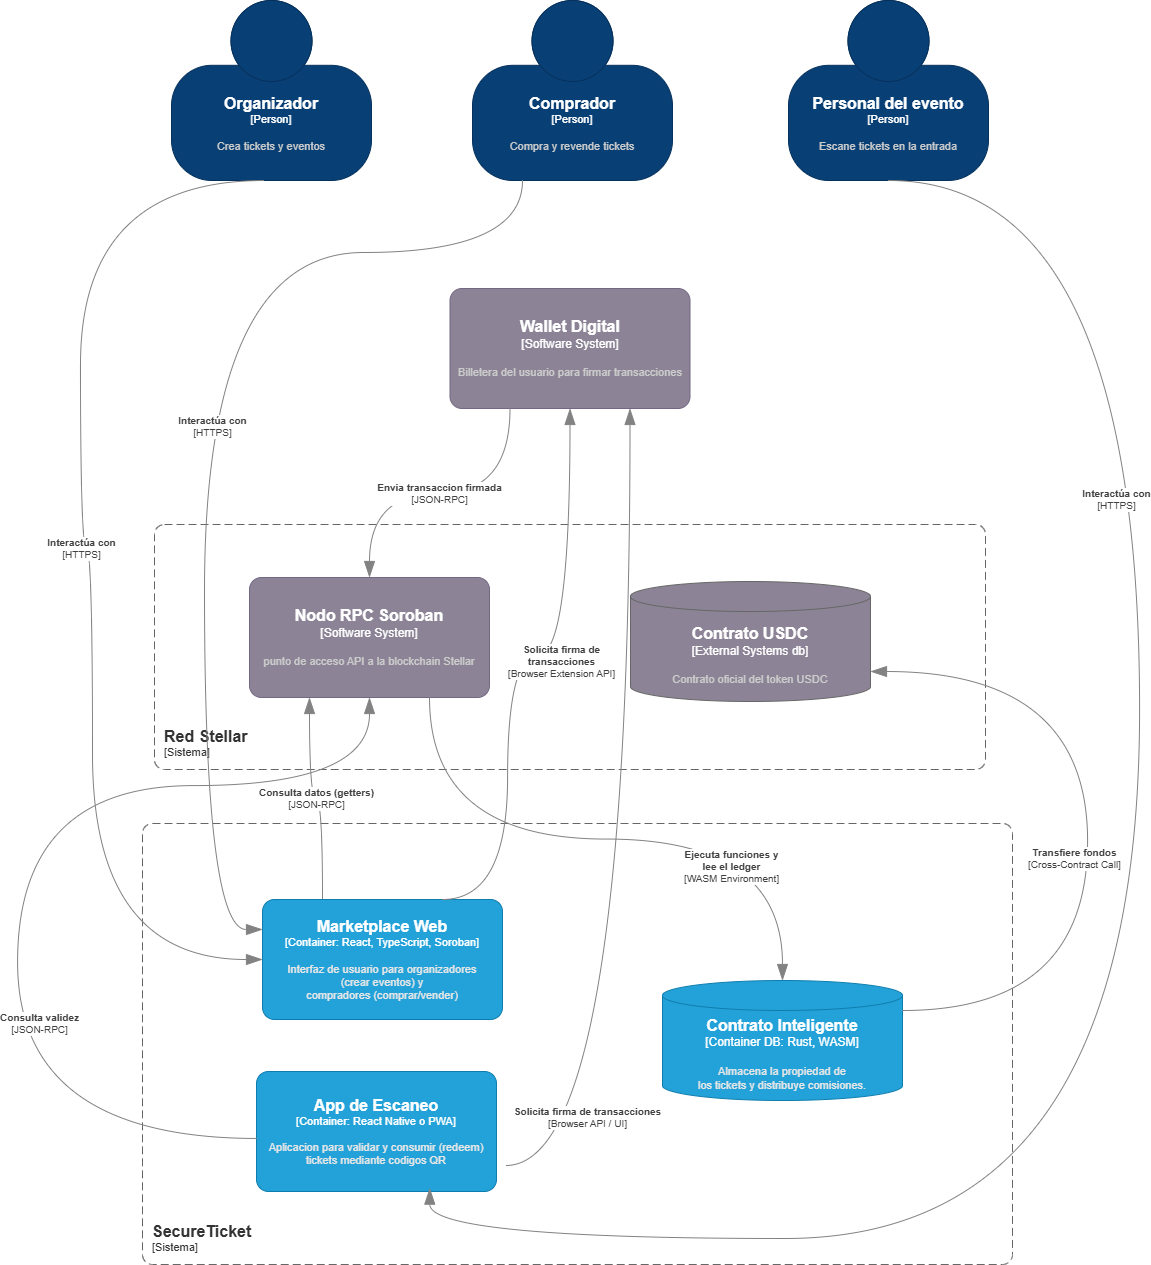
\includegraphics[width=0.7\textwidth]{ContenedoresSecureTicket.png}
  \caption{Diagrama C4 Nivel 2 -- Contenedores del sistema Stellar Tickets}
  \label{fig:c4-contenedores}
\end{figure}

\paragraph{Interpretación del diagrama.} El sistema se descompone en los siguientes contenedores, organizados en cuatro zonas:

\textbf{Zona Cliente} (lo que ejecuta el usuario en su dispositivo):
\begin{itemize}
  \item \textbf{Marketplace Web}: aplicación frontend (React/Next.js) que los organizadores, compradores y vendedores utilizan para interactuar con el sistema. Es una interfaz white-label, lo que significa que cada ticketera puede personalizarla con su marca.
  \item \textbf{App de Escaneo}: aplicación utilizada por el personal del evento para validar tickets mediante lectura de códigos QR. Opera tanto en modo online (consultando al backend en tiempo real) como en modo offline (con validación local y sincronización posterior).
  \item \textbf{Wallet Digital} (Freighter): componente externo al sistema que firma las transacciones antes de enviarlas a la blockchain.
\end{itemize}

\textbf{Zona Servidor} (lo que se ejecuta en la infraestructura de la plataforma):
\begin{itemize}
  \item \textbf{Nodo RPC Soroban}: punto de acceso a la red Stellar que permite al backend enviar transacciones y consultar el estado de los contratos. Actúa como puente entre el mundo off-chain y la blockchain.
\end{itemize}

\textbf{Zona Blockchain} (Stellar Testnet, lo que se ejecuta de forma descentralizada):
\begin{itemize}
  \item \textbf{Contrato Inteligente}: contrato Soroban desplegado por evento que contiene toda la lógica de negocio on-chain: emisión de tickets como NFTs, transferencia de propiedad, distribución de comisiones y marcado de tickets como usados. Es el componente más crítico del sistema.
  \item \textbf{Contrato USDC}: contrato externo del token estable utilizado como medio de pago. El contrato inteligente lo invoca para ejecutar las transferencias de fondos durante compras y reventas.
\end{itemize}

\textbf{Comunicaciones clave} visibles en el diagrama:
\begin{itemize}
  \item El Marketplace Web se comunica con el Nodo RPC Soroban para enviar transacciones firmadas y consultar estado.
  \item El Marketplace Web interactúa con la Wallet Digital para solicitar firmas de transacciones al usuario.
  \item La App de Escaneo consulta el estado de tickets a través del Nodo RPC o de datos sincronizados localmente.
  \item El Contrato Inteligente invoca al Contrato USDC para procesar pagos de forma atómica dentro de la misma transacción.
  \item La Red Stellar subyace como infraestructura que persiste el estado de todos los contratos de forma inmutable y distribuida.
\end{itemize}

\newpage
\subsection{Mapeo de vistas a secciones del documento}

Las secciones restantes del SAD profundizan en aspectos específicos de la arquitectura, complementando los diagramas C4:

\begin{table}[H]
  \centering
  \begin{tabularx}{\textwidth}{@{}l l X@{}}
    \toprule
    \textbf{Vista} & \textbf{Sección} & \textbf{Contenido principal}\\
    \midrule
    Casos de uso & \ref{sec:vista-casos-uso} & Casos de uso arquitectónicamente significativos y diagrama C4 de contexto.\\
    Lógica & \ref{sec:vista-logica} & Descomposición en capas y módulos; diagrama C4 de contenedores; separación on-chain/off-chain.\\
    Procesos & \ref{sec:vista-procesos} & Flujos de interacción principales: compra primaria, reventa atómica, redención y verificación.\\
    Despliegue & \ref{sec:vista-despliegue} & Topología de nodos: presentación, servicios, datos y red Stellar testnet.\\
    Implementación & \ref{sec:vista-implementacion} & Organización del código fuente, artefactos compilados (WASM) y dependencias.\\
    Datos & \ref{sec:vista-datos} & Modelo de almacenamiento on-chain (Soroban) y off-chain (PostgreSQL).\\
    \bottomrule
  \end{tabularx}
  \caption{Mapeo entre vistas arquitectónicas y secciones del SAD}
  \label{tab:mapeo-vistas}
\end{table}

Adicionalmente, el documento incluye una sección de \textbf{atributos de calidad} (Sección~\ref{sec:calidad}) con escenarios y tácticas arquitectónicas, y un \textbf{registro de decisiones arquitectónicas} (Sección~\ref{sec:decisiones}) en formato ADR.

%===============================================================
\newpage
\section{Objetivos y restricciones arquitectónicas}
\label{sec:objetivos-restricciones}
%===============================================================

Esta sección presenta los \textit{drivers} arquitectónicos: los atributos de calidad prioritarios y las restricciones que condicionan las decisiones de diseño del sistema.

\subsection{Objetivos arquitectónicos}
\label{subsec:objetivos}

Los siguientes atributos de calidad, derivados del SRS y de las necesidades del modelo B2B, guían las decisiones arquitectónicas:

\begin{enumerate}
  \item \textbf{Trazabilidad e inmutabilidad.} Cada ticket debe tener un historial de propiedad verificable e inalterable. Esto motiva el uso de blockchain como fuente de verdad para la propiedad y las transferencias, complementado con un indexador off-chain para consultas rápidas.

  \item \textbf{Atomicidad en transacciones de reventa.} La operación de compra en el mercado secundario debe ser atómica: la transferencia del ticket y la distribución de pagos (vendedor, comisión organizador, comisión plataforma) ocurren en una sola transacción o no ocurren en absoluto. Esto elimina estados inconsistentes donde el pago se procesa pero el ticket no se transfiere, o viceversa.

  \item \textbf{Seguridad y autenticidad.} La arquitectura debe garantizar que los tickets no puedan falsificarse ni duplicarse. La custodia de claves es no-custodial (Freighter Wallet), de modo que solo el propietario legítimo puede autorizar transferencias mediante firma criptográfica.

  \item \textbf{Adaptabilidad B2B (multi-ticketera).} El sistema debe permitir que múltiples ticketeras operen de forma independiente, cada una con sus propios eventos, políticas de comisión y configuración. Esto motiva la arquitectura de \textit{contrato por evento} desplegado por un Factory, y un frontend white-label configurable.

  \item \textbf{Disponibilidad de consultas.} Aunque la blockchain garantiza persistencia, su modelo de lectura es limitado. El sistema debe ofrecer consultas rápidas sobre estado de tickets, historial y auditoría sin depender exclusivamente de llamadas on-chain. Esto justifica la capa de indexación y caché off-chain respaldada por PostgreSQL.

  \item \textbf{Verificabilidad en puerta.} La validación de tickets en el punto de acceso al evento debe funcionar tanto en modo online (consulta directa al contrato) como offline (con sincronización posterior), para cubrir escenarios donde la conectividad es limitada.
\end{enumerate}

\subsection{Restricciones arquitectónicas}
\label{subsec:restricciones}

\subsubsection{Restricciones tecnológicas}

\begin{itemize}
  \item \textbf{Stellar y Soroban:} la lógica on-chain debe implementarse como contratos inteligentes Soroban, compilados a WebAssembly (WASM) y escritos en Rust. Esto impone el uso del \texttt{soroban-sdk} y sus limitaciones (modelo de storage basado en claves, sin eventos complejos nativos, tamaño limitado de transacciones).
  \item \textbf{Testnet:} el prototipo opera exclusivamente sobre la testnet de Stellar, lo que implica que los activos no tienen valor monetario real y que la red puede presentar interrupciones o reinicios periódicos.
  \item \textbf{Token de pago:} las transacciones de compra y reventa utilizan XLM nativo y, opcionalmente, un token USDC simulado (\texttt{USDC\_SIM}) emitido en testnet mediante el Stellar Asset Contract (SAC).
  \item \textbf{Wallet no-custodial:} el sistema no almacena claves privadas de los usuarios. La firma de transacciones se delega a Freighter Wallet, lo que requiere que el frontend integre su SDK para la interacción con el usuario.
\end{itemize}

\subsubsection{Restricciones organizacionales}

\begin{itemize}
  \item \textbf{Equipo reducido:} 4 desarrolladores con dedicación parcial (proyecto académico), lo que favorece una arquitectura con separación clara de responsabilidades que permita trabajo en paralelo (contrato, backend, frontend, verificación).
  \item \textbf{Tiempo acotado:} dos semestres académicos ($\sim$32 semanas), lo que limita el alcance a un prototipo funcional demostrable.
  \item \textbf{Contexto académico:} el sistema debe ser documentable, demostrable y evaluable por docentes, priorizando claridad arquitectónica sobre optimización de producción.
\end{itemize}

\subsubsection{Restricciones de integración}

\begin{itemize}
  \item \textbf{Modelo B2B no invasivo:} el sistema se ofrece como complemento a plataformas de boletería existentes, no como reemplazo. La integración se realiza vía API REST, sin requerir modificaciones en los sistemas internos de la ticketera.
  \item \textbf{Separación on-chain/off-chain:} las operaciones de escritura que afectan propiedad y pagos ocurren on-chain (fuente de verdad), mientras que las consultas de lectura, auditoría e indexación se resuelven off-chain para rendimiento y usabilidad.
\end{itemize}

%===============================================================
\newpage
\section{Vista de casos de uso}
\label{sec:vista-casos-uso}
%===============================================================

Esta sección identifica los casos de uso arquitectónicamente significativos del sistema: aquellos que ejercitan los principales componentes, imponen restricciones de diseño o exponen los atributos de calidad prioritarios descritos en la Sección~\ref{sec:objetivos-restricciones}.

\subsection{Diagrama de casos de uso}

La Figura~\ref{fig:casos-uso} presenta los casos de uso principales del sistema y sus relaciones con los actores identificados en el diagrama C4 de contexto (Figura~\ref{fig:c4-contexto}).

\begin{figure}[H]
  \centering
  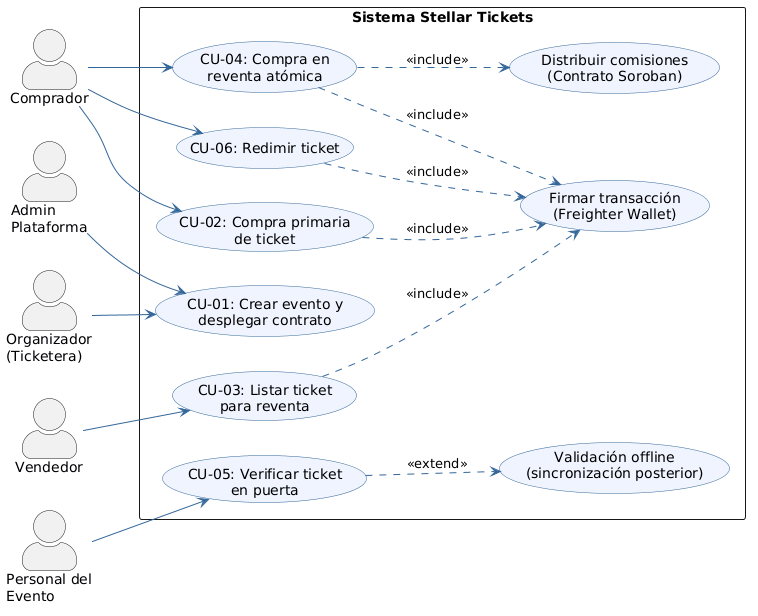
\includegraphics[width=0.7\textwidth]{CasosDeUso_SAD.png}
  \caption{Diagrama de casos de uso arquitectónicamente significativos}
  \label{fig:casos-uso}
\end{figure}

\subsection{Descripción de casos de uso}

A continuación se describe cada caso de uso, destacando su relevancia arquitectónica.

\subsubsection{CU-01: Crear evento y desplegar contrato}

\begin{table}[H]
  \centering
  \begin{tabularx}{\textwidth}{@{}p{3.5cm} X@{}}
    \toprule
    \textbf{Actores} & Organizador (Ticketera), Admin Plataforma\\
    \midrule
    \textbf{Descripción} & El organizador configura un nuevo evento (nombre, fecha, wallets de comisión, políticas de reventa). La plataforma invoca el Factory para desplegar un contrato Soroban específico para ese evento en la testnet.\\
    \midrule
    \textbf{Precondiciones} & El organizador está autenticado y tiene permisos de creación de eventos.\\
    \midrule
    \textbf{Flujo principal} &
      1. El organizador ingresa los datos del evento y configura fees.\newline
      2. El backend valida los parámetros y registra el evento en PostgreSQL.\newline
      3. El backend invoca el contrato Factory en Stellar.\newline
      4. El Factory despliega un nuevo contrato de evento con los parámetros configurados.\newline
      5. El sistema registra la dirección del contrato desplegado.\\
    \midrule
    \textbf{Postcondiciones} & Existe un contrato de evento independiente en la testnet, listo para emitir tickets.\\
    \midrule
    \textbf{Relevancia arquitectónica} & Ejerce el patrón Factory, la separación on-chain/off-chain y la adaptabilidad multi-ticketera. Cada evento opera con un contrato aislado, lo que garantiza independencia de configuración y fondos.\\
    \bottomrule
  \end{tabularx}
  \caption{CU-01: Crear evento y desplegar contrato}
  \label{tab:cu01}
\end{table}

\subsubsection{CU-02: Compra primaria de ticket}

\begin{table}[H]
  \centering
  \begin{tabularx}{\textwidth}{@{}p{3.5cm} X@{}}
    \toprule
    \textbf{Actores} & Comprador\\
    \midrule
    \textbf{Descripción} & El comprador adquiere un ticket emitido por el organizador. El 100\% del pago se transfiere al organizador.\\
    \midrule
    \textbf{Precondiciones} & El evento existe, tiene tickets disponibles y el comprador tiene fondos suficientes en su wallet.\\
    \midrule
    \textbf{Flujo principal} &
      1. El comprador selecciona un ticket disponible en el marketplace.\newline
      2. El frontend solicita firma de la transacción a Freighter Wallet.\newline
      3. El contrato de evento transfiere el pago al organizador y asigna el ticket al comprador.\newline
      4. El indexador registra la operación en PostgreSQL.\\
    \midrule
    \textbf{Postcondiciones} & El comprador es el nuevo propietario del ticket. El pago fue transferido al organizador.\\
    \midrule
    \textbf{Relevancia arquitectónica} & Ejerce la integración wallet no-custodial (Freighter), el flujo de firma de transacciones y la escritura on-chain con indexación off-chain posterior.\\
    \bottomrule
  \end{tabularx}
  \caption{CU-02: Compra primaria de ticket}
  \label{tab:cu02}
\end{table}

\subsubsection{CU-03: Listar ticket para reventa}

\begin{table}[H]
  \centering
  \begin{tabularx}{\textwidth}{@{}p{3.5cm} X@{}}
    \toprule
    \textbf{Actores} & Vendedor\\
    \midrule
    \textbf{Descripción} & El propietario de un ticket lo publica en el marketplace para reventa, estableciendo un precio.\\
    \midrule
    \textbf{Precondiciones} & El vendedor es propietario del ticket, el ticket está vigente (no consumido ni invalidado) y el evento permite reventa.\\
    \midrule
    \textbf{Flujo principal} &
      1. El vendedor selecciona un ticket de su inventario y fija precio de reventa.\newline
      2. El frontend solicita firma a Freighter Wallet.\newline
      3. El contrato marca el ticket como listado para reventa.\newline
      4. El marketplace muestra el ticket disponible para compra.\\
    \midrule
    \textbf{Postcondiciones} & El ticket está visible en el marketplace con estado \texttt{for\_sale = true}.\\
    \midrule
    \textbf{Relevancia arquitectónica} & Ejerce la transición de estados del ticket on-chain y la sincronización con el caché off-chain para consultas del marketplace.\\
    \bottomrule
  \end{tabularx}
  \caption{CU-03: Listar ticket para reventa}
  \label{tab:cu03}
\end{table}

\subsubsection{CU-04: Compra en reventa atómica}

\begin{table}[H]
  \centering
  \begin{tabularx}{\textwidth}{@{}p{3.5cm} X@{}}
    \toprule
    \textbf{Actores} & Comprador\\
    \midrule
    \textbf{Descripción} & El comprador adquiere un ticket en el mercado secundario. En una sola transacción atómica se ejecutan: pago al vendedor, comisión al organizador, comisión a la plataforma, burn de la versión anterior y mint de una nueva versión del ticket.\\
    \midrule
    \textbf{Precondiciones} & El ticket está listado para reventa, el comprador tiene fondos suficientes y no es el propietario actual.\\
    \midrule
    \textbf{Flujo principal} &
      1. El comprador selecciona un ticket en reventa y confirma la compra.\newline
      2. Freighter Wallet firma la transacción.\newline
      3. El contrato ejecuta atómicamente:\newline
      \hspace{1em}a) Transferencia de comisión al organizador.\newline
      \hspace{1em}b) Transferencia de comisión a la plataforma.\newline
      \hspace{1em}c) Transferencia del pago neto al vendedor.\newline
      \hspace{1em}d) Burn de la versión previa del ticket.\newline
      \hspace{1em}e) Mint de nueva versión asignada al comprador.\newline
      4. El contrato emite evento on-chain indexado por \texttt{ticket\_root\_id}.\newline
      5. El indexador actualiza PostgreSQL.\\
    \midrule
    \textbf{Flujo alternativo} & Si cualquier paso falla, toda la transacción se revierte. No existe estado intermedio.\\
    \midrule
    \textbf{Postcondiciones} & El comprador posee la nueva versión del ticket. Los pagos y comisiones fueron distribuidos. La versión anterior está invalidada.\\
    \midrule
    \textbf{Relevancia arquitectónica} & Es el caso de uso más crítico del sistema. Ejerce la atomicidad transaccional de Soroban, el patrón burn+remint, la distribución de comisiones embebida en el contrato y la trazabilidad por \texttt{ticket\_root\_id}. Valida el driver de atomicidad e inmutabilidad.\\
    \bottomrule
  \end{tabularx}
  \caption{CU-04: Compra en reventa atómica}
  \label{tab:cu04}
\end{table}

\subsubsection{CU-05: Verificar ticket en puerta}

\begin{table}[H]
  \centering
  \begin{tabularx}{\textwidth}{@{}p{3.5cm} X@{}}
    \toprule
    \textbf{Actores} & Personal del Evento\\
    \midrule
    \textbf{Descripción} & El verificador escanea el código QR del ticket para validar el acceso al evento. Soporta modo online y offline.\\
    \midrule
    \textbf{Precondiciones} & El ticket existe y el evento está en curso o próximo a iniciar.\\
    \midrule
    \textbf{Flujo principal (online)} &
      1. El asistente presenta el QR (contiene ticket ID, versión, firma y expiración).\newline
      2. La app de verificación consulta el backend.\newline
      3. El backend valida contra el caché de estado y opcionalmente contra el contrato on-chain.\newline
      4. Se confirma o deniega el acceso.\newline
      5. Se registra el check-in en la bitácora.\\
    \midrule
    \textbf{Flujo alternativo (offline)} &
      1. Sin conectividad, la app aplica validación local con datos sincronizados previamente.\newline
      2. El resultado se marca como provisional.\newline
      3. Al recuperar conectividad, se sincronizan los consumos pendientes.\newline
      4. Conflictos se resuelven por política: primer check-in sincronizado gana.\\
    \midrule
    \textbf{Postcondiciones} & El ticket queda marcado como consumido (online) o pendiente de sincronización (offline).\\
    \midrule
    \textbf{Relevancia arquitectónica} & Ejerce la táctica de resiliencia offline, la cola de sincronización, la resolución de conflictos y la separación entre validación on-chain y caché off-chain. Valida el driver de verificabilidad en puerta.\\
    \bottomrule
  \end{tabularx}
  \caption{CU-05: Verificar ticket en puerta}
  \label{tab:cu05}
\end{table}

\subsubsection{CU-06: Redimir ticket}

\begin{table}[H]
  \centering
  \begin{tabularx}{\textwidth}{@{}p{3.5cm} X@{}}
    \toprule
    \textbf{Actores} & Comprador\\
    \midrule
    \textbf{Descripción} & El propietario del ticket lo redime, marcándolo como usado de forma irreversible en el contrato.\\
    \midrule
    \textbf{Precondiciones} & El ticket está vigente, no está listado para reventa y el actor es el propietario.\\
    \midrule
    \textbf{Flujo principal} &
      1. El comprador solicita la redención del ticket.\newline
      2. Freighter Wallet firma la transacción.\newline
      3. El contrato marca el ticket como \texttt{used = true} (irreversible).\newline
      4. El indexador actualiza el estado en PostgreSQL.\\
    \midrule
    \textbf{Postcondiciones} & El ticket no puede ser listado, comprado ni revendido. El estado es terminal.\\
    \midrule
    \textbf{Relevancia arquitectónica} & Ejerce la irreversibilidad de estado on-chain y la transición terminal en la máquina de estados del ticket.\\
    \bottomrule
  \end{tabularx}
  \caption{CU-06: Redimir ticket}
  \label{tab:cu06}
\end{table}

%===============================================================
\newpage
\section{Vista lógica}
\label{sec:vista-logica}
%===============================================================

Esta sección describe la descomposición lógica del sistema en capas y módulos, profundizando el diagrama C4 de contenedores (Figura~\ref{fig:c4-contenedores}). La separación fundamental es entre la lógica \textbf{on-chain} (ejecutada de forma descentralizada en la red Stellar) y la lógica \textbf{off-chain} (ejecutada en infraestructura controlada por la plataforma).

\subsection{Arquitectura en capas}

El sistema se organiza en cuatro capas lógicas, cada una con responsabilidades claramente delimitadas:

\begin{enumerate}
  \item \textbf{Capa de presentación} (Frontend): interfaz de usuario que permite a los distintos actores interactuar con el sistema.
  \item \textbf{Capa de servicios} (Backend/API): lógica de negocio off-chain, orquestación de operaciones, autenticación y exposición de endpoints.
  \item \textbf{Capa de datos} (PostgreSQL + Caché): persistencia off-chain para consultas rápidas, auditoría e indexación.
  \item \textbf{Capa blockchain} (Stellar/Soroban): lógica de negocio on-chain, fuente de verdad para propiedad de tickets y pagos.
\end{enumerate}

\begin{table}[H]
  \centering
  \begin{tabularx}{\textwidth}{@{}p{3cm} p{4cm} X@{}}
    \toprule
    \textbf{Capa} & \textbf{Contenedores} & \textbf{Responsabilidad}\\
    \midrule
    Presentación & Marketplace Web, App de Escaneo & Renderizar interfaces, capturar acciones del usuario, solicitar firma de transacciones a Freighter.\\
    Servicios & API REST, Módulo Auth, Módulo Reventa, Módulo Verificación QR, Indexador, Cola de sincronización & Autenticar usuarios, orquestar operaciones de negocio, indexar eventos on-chain, gestionar verificación online/offline.\\
    Datos & PostgreSQL, Bitácora de auditoría, Caché de estado de tickets & Persistir entidades de negocio, historial de transacciones, estado cacheado de tickets para consultas rápidas.\\
    Blockchain & Contrato Factory, Contrato por Evento, SAC XLM, Token USDC\_SIM & Emitir tickets (NFTs), transferir propiedad, distribuir comisiones, marcar tickets como usados. Fuente de verdad inmutable.\\
    \bottomrule
  \end{tabularx}
  \caption{Descomposición en capas lógicas}
  \label{tab:capas}
\end{table}

\subsection{Capa de presentación}

La capa de presentación se compone de dos aplicaciones cliente:

\subsubsection{Marketplace Web (React/Next.js)}

Aplicación web white-label que permite a cada ticketera personalizar la experiencia de marca. Expone las siguientes funcionalidades según el rol del usuario:

\begin{itemize}
  \item \textbf{Organizador}: creación de eventos, configuración de wallets de comisión y políticas de reventa, consulta de reportes.
  \item \textbf{Comprador/Vendedor}: visualización de tickets propios, publicación en el marketplace, compra de tickets en venta primaria o reventa, consulta de trazabilidad.
  \item \textbf{Admin Plataforma}: configuración de comisiones de la plataforma y monitoreo general.
\end{itemize}

La comunicación con la blockchain no es directa: el frontend solicita firma de transacciones a \textbf{Freighter Wallet} (SDK integrado) y envía las transacciones firmadas a través del Nodo RPC Soroban.

\subsubsection{App de Escaneo (Verificador)}

Aplicación dedicada al personal del evento para validar tickets mediante lectura de códigos QR. Soporta dos modos de operación:

\begin{itemize}
  \item \textbf{Modo online}: consulta al backend en tiempo real, que valida contra el caché y opcionalmente contra el estado on-chain.
  \item \textbf{Modo offline}: validación local con datos pre-sincronizados. Los resultados se marcan como provisionales y se sincronizan cuando se recupera la conectividad (ventana máxima de 30 minutos).
\end{itemize}

\subsection{Capa de servicios (Backend)}

El backend centraliza la lógica de negocio off-chain y se organiza en los siguientes módulos:

\subsubsection{API REST}

Punto de entrada principal para el frontend y para integraciones B2B con ticketeras externas. Expone endpoints para:

\begin{itemize}
  \item Gestión de usuarios y eventos.
  \item Consulta de tickets, listados de reventa e historial.
  \item Operaciones de compra y verificación.
\end{itemize}

\subsubsection{Módulo de Autenticación y Roles}

Gestiona la identidad de los usuarios y el control de acceso basado en roles (organizador, comprador/vendedor, verificador, admin plataforma). Se integra con PostgreSQL para persistir sesiones y permisos.

\subsubsection{Módulo de Reventa}

Orquesta las operaciones de listado y compra de tickets. En la compra, coordina la construcción de la transacción Soroban que se envía al usuario para firma. No ejecuta la transacción directamente: la firma es responsabilidad del usuario a través de su wallet.

\subsubsection{Módulo de Verificación QR}

Procesa las solicitudes de validación de la App de Escaneo. En modo online, consulta el caché de estado de tickets y opcionalmente el contrato on-chain. Gestiona la cola de sincronización para consumos realizados en modo offline.

\subsubsection{Indexador de Eventos Stellar}

Proceso que consume eventos emitidos por los contratos en la red Stellar y los persiste en PostgreSQL. Permite ofrecer consultas de historial, trazabilidad y auditoría sin depender de llamadas directas a la blockchain, resolviendo la limitación de lectura de Soroban.

\subsection{Capa de datos (Off-chain)}

La capa de datos off-chain se compone de:

\begin{itemize}
  \item \textbf{PostgreSQL}: almacena entidades de negocio (usuarios, ticketeras, eventos), versiones de tickets (\texttt{TICKET\_ROOT} y \texttt{TICKET\_VERSION}), transacciones de reventa, listados y check-ins. Es la fuente de datos para las consultas del frontend y los reportes.
  \item \textbf{Bitácora de auditoría}: registro de eventos del negocio con referencias a transacciones on-chain (\texttt{tx\_hash}), utilizado para reconciliación y trazabilidad.
  \item \textbf{Caché de estado de tickets}: almacén de acceso rápido con el estado actual de los tickets, actualizado por el indexador. Permite validaciones en puerta sin latencia de consulta a la blockchain.
\end{itemize}

\subsection{Capa blockchain (On-chain)}

La capa on-chain es la fuente de verdad del sistema para la propiedad de tickets y la ejecución de pagos. Se compone de:

\subsubsection{Contrato Factory}

Contrato Soroban responsable de desplegar un contrato independiente por cada evento. Esta decisión arquitectónica garantiza que cada evento opera con su propia configuración (comisiones, wallets de pago) y su propio espacio de almacenamiento, aislando completamente los fondos y políticas entre eventos y entre ticketeras.

\subsubsection{Contrato por Evento (\texttt{SecureTicketContract})}

Contrato Soroban que implementa toda la lógica de negocio on-chain para un evento específico. Su estructura interna se organiza de la siguiente forma:

\paragraph{Modelo de datos (Storage).} El contrato utiliza un almacenamiento basado en claves (\texttt{DataKey}) con los siguientes elementos:

\begin{itemize}
  \item \texttt{Ticket(u32)}: almacena el struct \texttt{Ticket} por ID. Cada ticket contiene: \texttt{id}, \texttt{event\_id}, \texttt{owner} (dirección del propietario), \texttt{price}, \texttt{for\_sale} (si está listado), \texttt{is\_resale} (si ya fue revendido al menos una vez) y \texttt{used} (si fue canjeado).
  \item \texttt{TicketCount}: contador autoincremental de tickets emitidos.
  \item \texttt{Organizer}, \texttt{Platform}: direcciones de la ticketera y de la plataforma SecureTicket.
  \item \texttt{Token}: dirección del contrato de token de pago (USDC).
  \item \texttt{OrgFee}, \texttt{PlatFee}: porcentajes de comisión para organizador y plataforma.
\end{itemize}

\paragraph{Funciones de escritura (state-changing).} Cada función está protegida por \texttt{require\_auth()} que verifica la firma del actor autorizado:

\begin{itemize}
  \item \texttt{initialize}: configura el contrato con las direcciones, token de pago y porcentajes de comisión. Solo puede ejecutarse una vez (guarda de re-inicialización). Requiere auth del organizador.
  \item \texttt{create\_ticket}: emite un nuevo ticket asignado al organizador. Requiere auth del organizador.
  \item \texttt{list\_ticket}: marca un ticket como en venta y actualiza su precio. Requiere auth del owner. Valida que el ticket no esté ya en venta ni haya sido usado.
  \item \texttt{cancel\_sale}: retira un ticket del marketplace. Requiere auth del owner.
  \item \texttt{buy\_ticket}: ejecuta la compra de un ticket. Implementa dos flujos en una sola transacción atómica:
    \begin{itemize}
      \item \textit{Compra primaria} (\texttt{is\_resale = false}): el 100\% del pago se transfiere al organizador mediante el \texttt{TokenClient}. Después de la primera compra, el ticket se marca como \texttt{is\_resale = true}.
      \item \textit{Reventa} (\texttt{is\_resale = true}): el pago se distribuye en tres transferencias atómicas: comisión al organizador (\texttt{OrgFee\%}), comisión a la plataforma (\texttt{PlatFee\%}) y el remanente al vendedor.
    \end{itemize}
    Requiere auth del comprador. Valida que el comprador no sea el propietario actual.
  \item \texttt{redeem\_ticket}: marca el ticket como \texttt{used = true} de forma irreversible. Requiere auth del owner. Un ticket usado no puede listarse ni comprarse.
\end{itemize}

\paragraph{Funciones de lectura (views).} No requieren autorización:

\begin{itemize}
  \item \texttt{get\_ticket}: retorna el struct completo de un ticket por ID.
  \item \texttt{get\_owner}: retorna la dirección del propietario de un ticket.
  \item \texttt{get\_resale\_tickets}: retorna todos los tickets en reventa (\texttt{for\_sale = true} y \texttt{is\_resale = true}).
  \item \texttt{get\_event\_tickets}: retorna todos los tickets de un evento específico.
\end{itemize}

\subsubsection{Contratos de token (SAC XLM y USDC\_SIM)}

Contratos externos que implementan el estándar de token de Stellar. El contrato de evento los invoca mediante \texttt{TokenClient} para ejecutar las transferencias de pago. El sistema soporta XLM nativo y opcionalmente un token USDC simulado en testnet.

\subsection{Separación on-chain / off-chain}

La siguiente tabla resume el criterio de distribución de responsabilidades entre ambas capas:

\begin{table}[H]
  \centering
  \begin{tabularx}{\textwidth}{@{}X l l@{}}
    \toprule
    \textbf{Responsabilidad} & \textbf{On-chain} & \textbf{Off-chain}\\
    \midrule
    Propiedad de tickets (quién es dueño) & \checkmark & Copia indexada\\
    Ejecución de pagos y comisiones & \checkmark & ---\\
    Emisión de tickets (mint) & \checkmark & Registro indexado\\
    Redención (marcar como usado) & \checkmark & Copia indexada\\
    Historial de transacciones detallado & Eventos mínimos & \checkmark\\
    Consultas de búsqueda y filtrado & --- & \checkmark\\
    Autenticación y roles de usuario & --- & \checkmark\\
    Auditoría y bitácora operativa & Referencia (tx\_hash) & \checkmark\\
    Verificación de acceso (check-in) & Consulta opcional & \checkmark\\
    \bottomrule
  \end{tabularx}
  \caption{Distribución de responsabilidades on-chain vs. off-chain}
  \label{tab:onchain-offchain}
\end{table}

El principio rector es: \textit{lo que afecta propiedad o dinero se ejecuta on-chain} (fuente de verdad inmutable), \textit{lo que requiere consultas rápidas o contexto de negocio se resuelve off-chain} (rendimiento y usabilidad).

%===============================================================
\newpage
\section{Vista de procesos}
\label{sec:vista-procesos}
%===============================================================

Esta sección describe los flujos de interacción principales del sistema, enfocándose en cómo los componentes colaboran en tiempo de ejecución para resolver los casos de uso críticos. Se documentan tres flujos y la máquina de estados que gobierna el ciclo de vida del ticket.

% ---- Flujo 1: Compra primaria ----
\subsection{Flujo de compra primaria}

La compra primaria es el primer flujo que ocurre sobre un ticket recién creado. Involucra al comprador, el frontend, el contrato de evento y el token de pago.

\begin{enumerate}
  \item El organizador ha creado previamente el evento y emitido tickets mediante \texttt{create\_ticket}. Cada ticket queda asignado al organizador con \texttt{for\_sale = false} y \texttt{is\_resale = false}.
  \item El organizador lista el ticket para venta primaria invocando \texttt{list\_ticket}, que establece \texttt{for\_sale = true} y el precio.
  \item El comprador visualiza el ticket en el Marketplace Web y selecciona la compra.
  \item El frontend construye la transacción Soroban (\texttt{buy\_ticket}) y solicita firma a Freighter Wallet.
  \item El comprador firma y la transacción se envía a la red Stellar.
  \item El contrato de evento ejecuta la lógica de compra primaria: como \texttt{is\_resale = false}, el 100\% del pago se transfiere al organizador mediante el \texttt{TokenClient}.
  \item El contrato actualiza el ticket: \texttt{owner = comprador}, \texttt{for\_sale = false}, \texttt{is\_resale = true} (todas las ventas futuras serán reventas).
  \item El indexador detecta la transacción on-chain y registra la operación en PostgreSQL.
\end{enumerate}

\textbf{Aspecto arquitectónico clave:} la compra primaria establece la transición de \texttt{is\_resale = false} a \texttt{true}, lo que determina el comportamiento de todas las transacciones futuras sobre ese ticket (activación del split de comisiones).

% ---- Flujo 2: Reventa atómica ----
\subsection{Flujo de reventa atómica}

La Figura~\ref{fig:seq-reventa} presenta el diagrama de secuencia completo de este flujo.

\begin{figure}[H]
  \centering
  
\includegraphics[width=0.8\textwidth]{04_secuencia_reventa_atomica.png}
  \caption{Diagrama de secuencia -- Reventa atómica con distribución de comisiones}
  \label{fig:seq-reventa}
\end{figure}

Este es el flujo más crítico del sistema desde el punto de vista arquitectónico. La reventa debe ser \textbf{atómica}: todas las operaciones (distribución de pagos y transferencia de propiedad) ocurren en una sola transacción de Soroban, o ninguna ocurre. No existe estado intermedio.

\begin{enumerate}
  \item \textbf{Publicación:} el vendedor (propietario actual) invoca \texttt{list\_ticket} con el nuevo precio. El contrato verifica que el vendedor es el owner (\texttt{require\_auth}), que el ticket no está ya en venta y que no ha sido usado. El ticket queda con \texttt{for\_sale = true}.
  \item \textbf{Compra:} el comprador selecciona el ticket en el marketplace e inicia la compra. El frontend construye la transacción \texttt{buy\_ticket} y la envía a Freighter para firma.
  \item \textbf{Ejecución atómica en el contrato:} como \texttt{is\_resale = true}, el contrato ejecuta la distribución de comisiones en una sola transacción:
    \begin{enumerate}[label=\alph*)]
      \item Calcula la comisión del organizador: \texttt{precio $\times$ OrgFee / 100}.
      \item Calcula la comisión de la plataforma: \texttt{precio $\times$ PlatFee / 100}.
      \item Calcula el pago neto al vendedor: \texttt{precio $-$ comisión\_org $-$ comisión\_plat}.
      \item Ejecuta tres transferencias mediante \texttt{TokenClient}: al organizador, a la plataforma y al vendedor.
      \item Actualiza el ticket: \texttt{owner = comprador}, \texttt{for\_sale = false}.
    \end{enumerate}
  \item \textbf{Indexación:} el indexador registra la transacción en PostgreSQL con el \texttt{tx\_hash} correspondiente.
  \item \textbf{Notificación:} el frontend muestra al comprador su nuevo ticket y notifica al vendedor que la venta se completó.
\end{enumerate}

\textbf{Garantía de atomicidad:} si cualquiera de las transferencias de pago falla (por ejemplo, fondos insuficientes del comprador), toda la transacción se revierte automáticamente por el runtime de Soroban. Esto elimina por diseño los estados inconsistentes donde el pago se procesa pero el ticket no se transfiere, o viceversa. No se requiere lógica de compensación ni rollback manual.

% ---- Flujo 3: Verificación en puerta ----
\subsection{Flujo de verificación en puerta}

La verificación de acceso al evento es el flujo que ejerce la táctica de resiliencia offline del sistema. Soporta dos modos de operación según la disponibilidad de conectividad. La Figura~\ref{fig:seq-verificacion} presenta el diagrama de secuencia de ambos modos.

\begin{figure}[H]
  \centering
  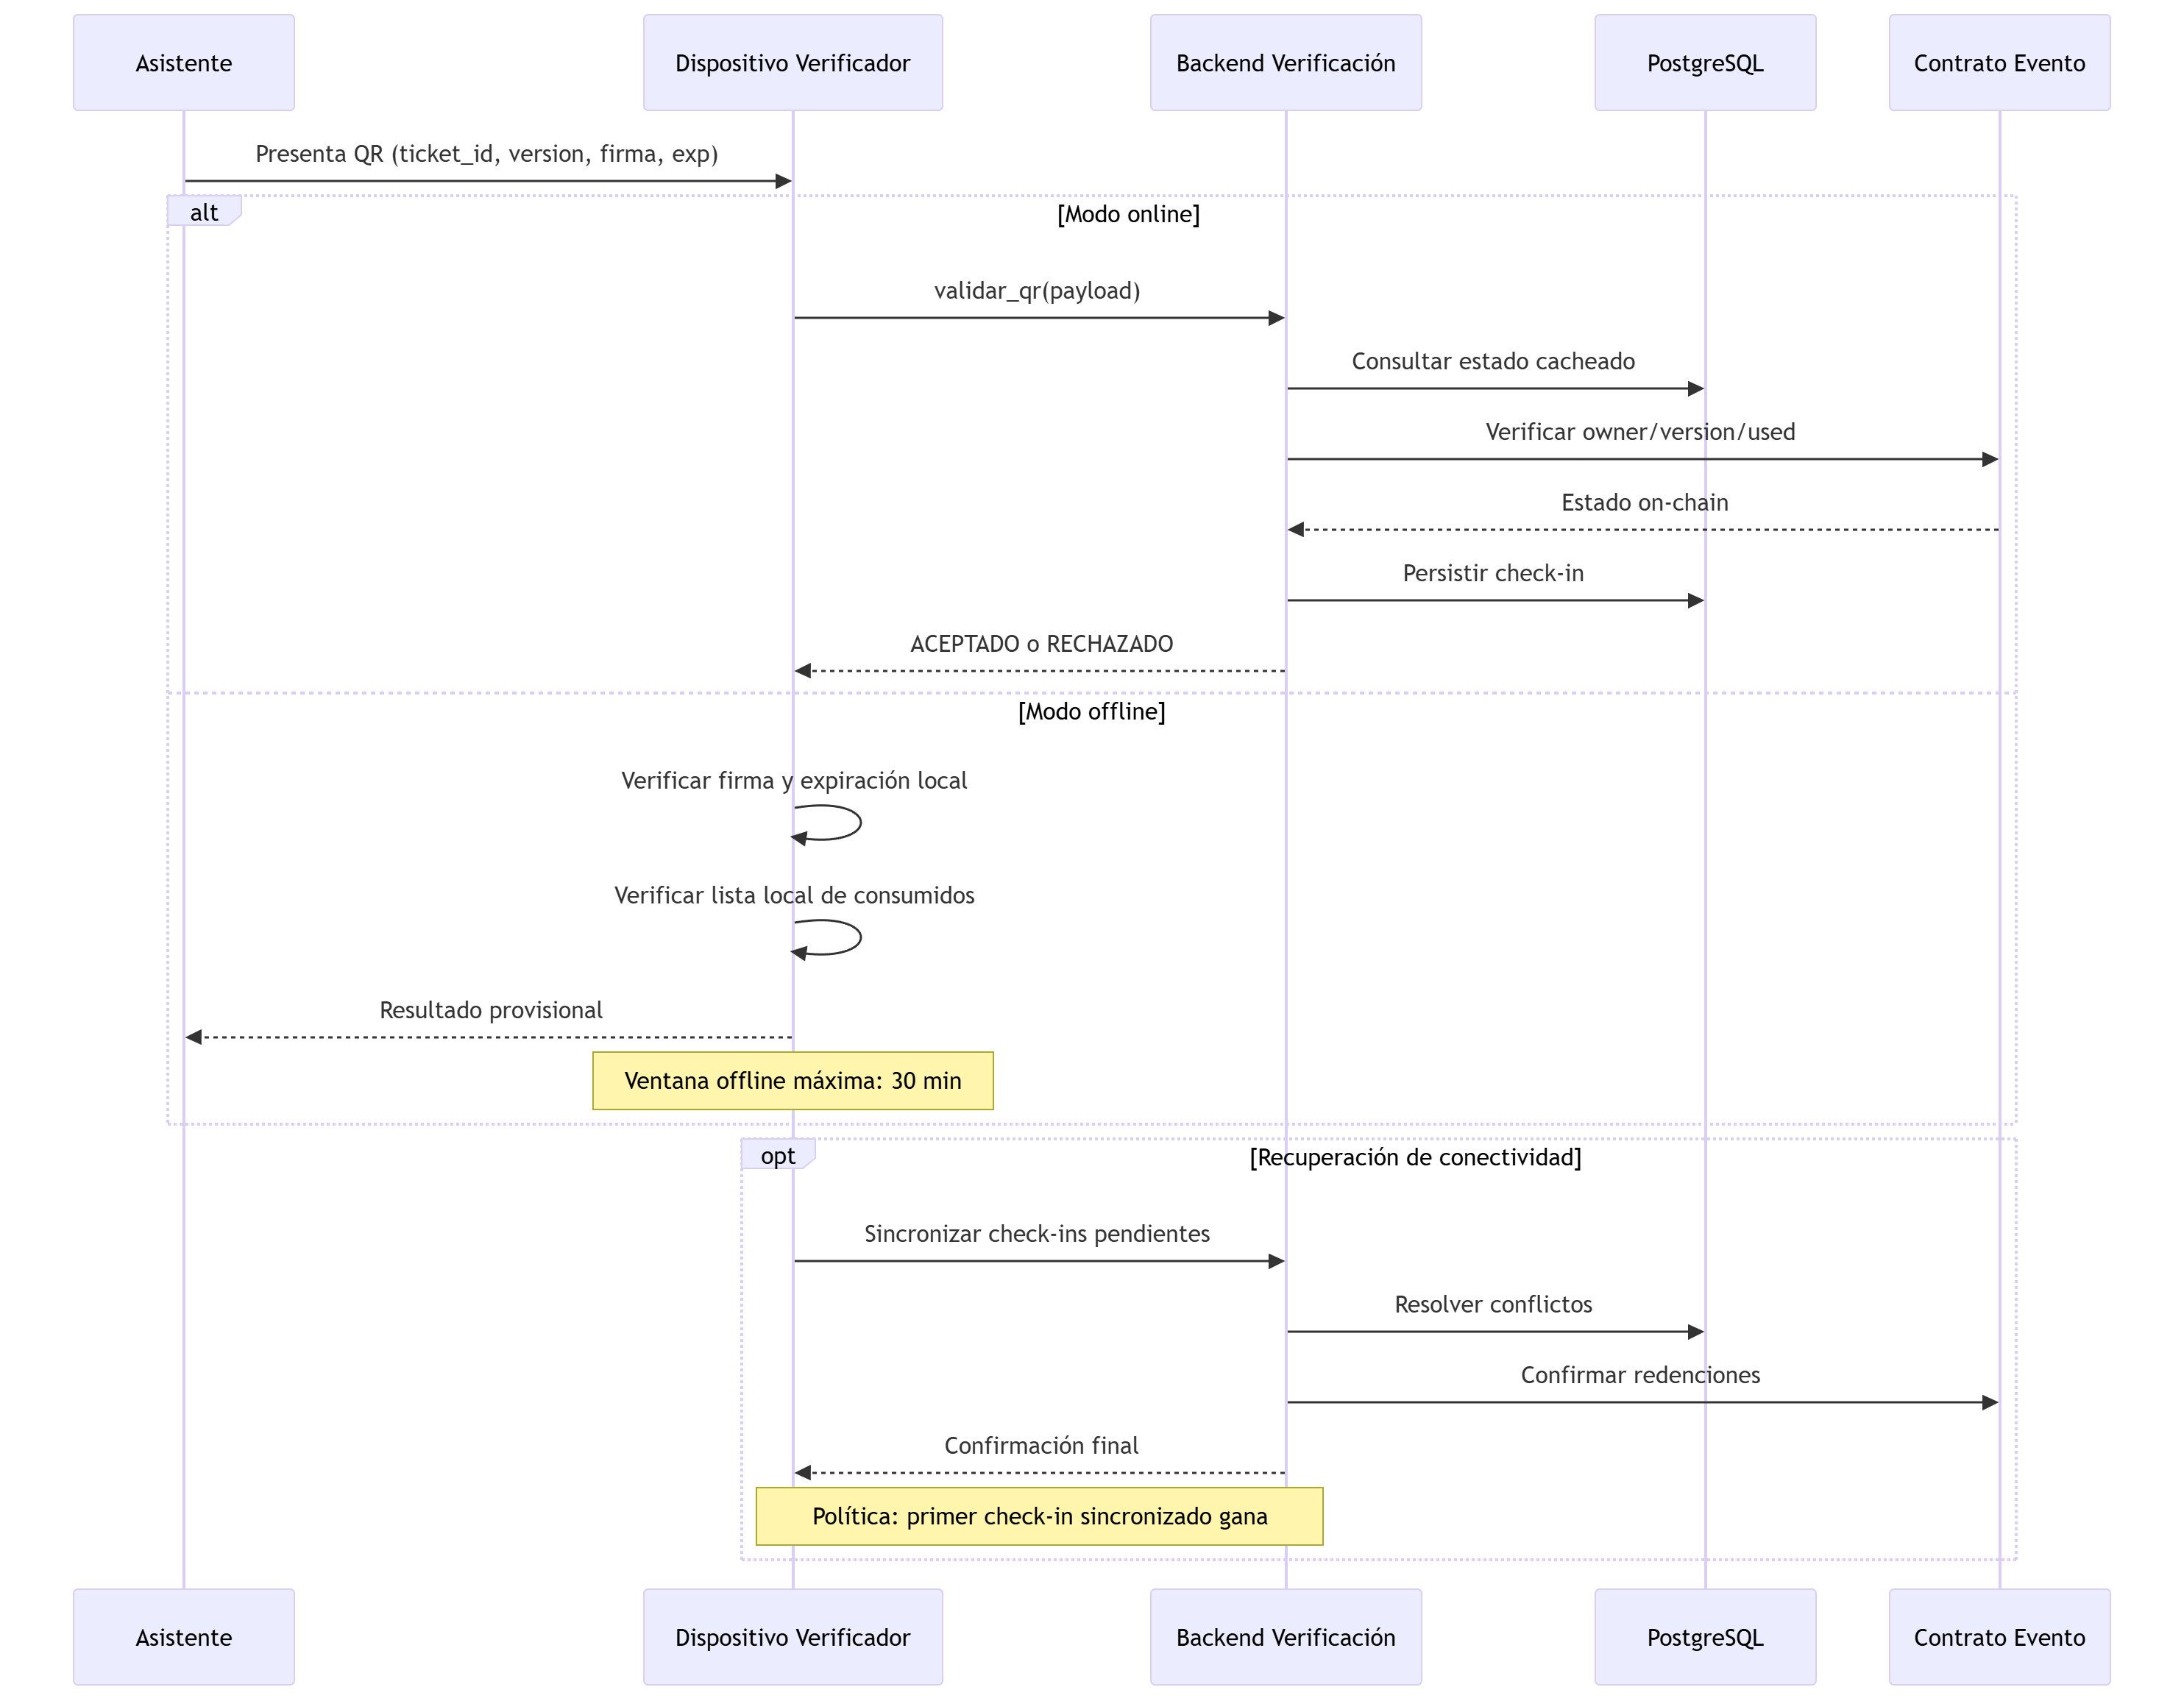
\includegraphics[width=0.8\textwidth]{05_secuencia_verificacion_online_offline.png}
  \caption{Diagrama de secuencia -- Verificación de ticket en puerta (online y offline)}
  \label{fig:seq-verificacion}
\end{figure}

\subsubsection{Modo online}

\begin{enumerate}
  \item El asistente presenta un código QR que contiene: \texttt{ticket\_id}, versión, firma criptográfica y timestamp de expiración.
  \item El dispositivo verificador (App de Escaneo) envía el payload al backend de verificación.
  \item El backend consulta el caché de estado de tickets en PostgreSQL para una respuesta rápida.
  \item Opcionalmente, el backend verifica directamente contra el contrato on-chain (consultando \texttt{owner}, versión y \texttt{used}).
  \item El backend persiste el check-in en la bitácora de auditoría y responde al verificador con ACEPTADO o RECHAZADO.
  \item Si se acepta, el ticket puede marcarse como consumido mediante \texttt{redeem\_ticket} en el contrato.
\end{enumerate}

\subsubsection{Modo offline}

En escenarios de conectividad limitada (eventos masivos, locaciones con cobertura deficiente), la App de Escaneo opera con datos pre-sincronizados:

\begin{enumerate}
  \item El dispositivo verificador valida localmente: verifica la firma criptográfica del QR, comprueba que no haya expirado y contrasta contra la lista local de tickets ya consumidos.
  \item El resultado se marca como \textbf{provisional} y se almacena localmente en el dispositivo.
  \item La ventana máxima de operación offline es de \textbf{30 minutos}. Después de este período, el dispositivo debe sincronizarse para seguir operando.
  \item Al recuperar conectividad, el dispositivo envía todos los check-ins pendientes al backend.
  \item El backend resuelve conflictos (por ejemplo, dos dispositivos aceptaron el mismo ticket en offline) aplicando la política: \textbf{primer check-in sincronizado gana}.
  \item Los conflictos resueltos se registran en la bitácora de auditoría para revisión posterior.
\end{enumerate}

\textbf{Aspecto arquitectónico clave:} la cola de sincronización y la política de resolución de conflictos son las tácticas que permiten al sistema operar en condiciones degradadas sin sacrificar la integridad. La autoridad de verificación es compartida entre el verificador (validación local provisional) y el backend (confirmación definitiva).

% ---- Máquina de estados ----
\subsection{Máquina de estados del ticket}

El ciclo de vida de un ticket está gobernado por una máquina de estados que define las transiciones válidas entre estados y las condiciones bajo las cuales pueden ocurrir. Esta máquina se implementa implícitamente en el contrato Soroban mediante las validaciones en cada función. La Figura~\ref{fig:estados-ticket} presenta el diagrama de estados completo.

\begin{figure}[H]
  \centering
  
\includegraphics[width=0.5\textwidth]{06_estados_ticket.png}
  \caption{Máquina de estados del ciclo de vida de un ticket}
  \label{fig:estados-ticket}
\end{figure}

\subsubsection{Estados}

\begin{table}[H]
  \centering
  \begin{tabularx}{\textwidth}{@{}p{3.5cm} X@{}}
    \toprule
    \textbf{Estado} & \textbf{Descripción}\\
    \midrule
    \textbf{Emitido} & El ticket acaba de ser creado por el organizador (\texttt{create\_ticket}). Está asignado al organizador, con \texttt{for\_sale = false}, \texttt{is\_resale = false}, \texttt{used = false}.\\
    \textbf{En venta} & El ticket ha sido listado para venta o reventa (\texttt{list\_ticket}). \texttt{for\_sale = true}. Visible en el marketplace.\\
    \textbf{Asignado} & El ticket tiene un propietario (comprador) y no está en venta. \texttt{for\_sale = false}. El propietario puede listarlo para reventa o asistir al evento.\\
    \textbf{Consumido} & El ticket fue redimido (\texttt{redeem\_ticket}). \texttt{used = true}. Estado terminal e irreversible. No puede listarse ni comprarse.\\
    \textbf{Invalidado} & El ticket fue cancelado por política del organizador o por cancelación del evento. Estado terminal (manejado off-chain en la versión actual del prototipo).\\
    \bottomrule
  \end{tabularx}
  \caption{Estados del ciclo de vida de un ticket}
  \label{tab:estados-ticket}
\end{table}

\subsubsection{Transiciones}

\begin{table}[H]
  \centering
  \begin{tabularx}{\textwidth}{@{}p{3cm} p{3cm} p{3.5cm} X@{}}
    \toprule
    \textbf{Desde} & \textbf{Hacia} & \textbf{Acción} & \textbf{Condiciones}\\
    \midrule
    Emitido & En venta & \texttt{list\_ticket} & El organizador (owner) lista el ticket para venta primaria.\\
    En venta & Asignado & \texttt{buy\_ticket} & Un comprador adquiere el ticket. En venta primaria, \texttt{is\_resale} pasa a \texttt{true}.\\
    Asignado & En venta & \texttt{list\_ticket} & El propietario lista el ticket para reventa. El ticket debe no estar usado.\\
    En venta & Asignado & \texttt{cancel\_sale} & El propietario retira el ticket del marketplace.\\
    En venta & Asignado & \texttt{buy\_ticket} & En reventa: se ejecuta distribución de comisiones y transferencia de propiedad.\\
    Asignado & Consumido & \texttt{redeem\_ticket} & El propietario redime el ticket. Transición irreversible (\texttt{used = true}).\\
    Cualquiera & Invalidado & Política off-chain & Cancelación del evento o decisión del organizador. Gestionado por el backend.\\
    \bottomrule
  \end{tabularx}
  \caption{Transiciones válidas entre estados del ticket}
  \label{tab:transiciones-ticket}
\end{table}

\subsubsection{Reglas de integridad}

Las siguientes reglas son impuestas por el contrato y no pueden ser violadas:

\begin{itemize}
  \item Un ticket con \texttt{used = true} no puede cambiar a ningún otro estado. La redención es \textbf{irreversible}.
  \item Un ticket con \texttt{for\_sale = true} no puede ser redimido (debe cancelarse la venta primero).
  \item Solo el \texttt{owner} actual puede invocar \texttt{list\_ticket}, \texttt{cancel\_sale} y \texttt{redeem\_ticket} (verificado por \texttt{require\_auth}).
  \item Un propietario no puede comprarse su propio ticket (\texttt{self\_buy} está prohibido).
  \item El contrato solo puede inicializarse una vez (guarda de re-inicialización).
  \item Las comisiones de organizador y plataforma no pueden sumar 100\% o más del precio.
\end{itemize}

%===============================================================
\newpage
\section{Vista de despliegue}
\label{sec:vista-despliegue}
%===============================================================

% TODO: Diagrama de despliegue (nodos físicos/virtuales).
% Stellar testnet, servidor backend, hosting frontend, base de datos.

%===============================================================
\newpage
\section{Vista de implementación}
\label{sec:vista-implementacion}
%===============================================================

% TODO: Organización del código fuente, módulos, dependencias.
% Estructura del repositorio, artefactos compilados (WASM).

%===============================================================
\newpage
\section{Vista de datos}
\label{sec:vista-datos}
%===============================================================

% TODO: Modelo de datos on-chain (DataKey, Ticket struct, storage).
% Modelo de datos off-chain (si aplica: PostgreSQL, tablas).
% Diagrama entidad-relación o equivalente.

%===============================================================
\newpage
\section{Atributos de calidad}
\label{sec:calidad}
%===============================================================

% TODO: Escenarios de atributos de calidad (seguridad, rendimiento,
% disponibilidad, modificabilidad, etc.) y tácticas arquitectónicas
% empleadas para satisfacerlos.

%===============================================================
\newpage
\section{Decisiones arquitectónicas}
\label{sec:decisiones}
%===============================================================

% TODO: ADRs (Architecture Decision Records).
% Formato sugerido por decisión:
% - Contexto
% - Decisión
% - Consecuencias
% Ejemplos: elección de Stellar/Soroban, modelo de storage del contrato,
% separación on-chain/off-chain, stack de frontend/backend.

%===============================================================
% Referencias (si se usa bibliografía adicional al final)
%===============================================================

\end{document}
